\documentclass[a4, 12pt]{article}
\usepackage[a4paper,top=1.3cm,bottom=2cm,left=1.5cm,right=1.5cm,marginparwidth=0.75cm]{geometry}
\usepackage{setspace}
\usepackage{cmap}
\usepackage{mathtext}
\usepackage[utf8]{inputenc}
\usepackage[english,russian]{babel}
\usepackage[T2A]{fontenc}
\usepackage{multirow}
\usepackage{graphicx}
\usepackage{wrapfig}
\usepackage{tabularx}
\usepackage{float}
\usepackage{longtable}
\usepackage{hyperref}
\hypersetup{colorlinks=true,urlcolor=blue}
\usepackage[rgb]{xcolor}
\usepackage{amsmath,amsfonts,amssymb,amsthm,mathtools}
\usepackage{icomma}
\mathtoolsset{showonlyrefs=true}
\usepackage{euscript}
\usepackage{mathrsfs}

\DeclareMathOperator{\sgn}{\mathop{sgn}}
\newcommand*{\hm}[1]{#1\nobreak\discretionary{}
	{\hbox{$\mathsurround=0pt #1$}}{}}


\title{\textbf{Определение моментов инерции твердых тел с помощью трифилярного подвеса. (1.2.3)}}
\author{Дудаков Семён Б01-303}
\date{30 октября 2023}


\begin{document}

	\maketitle

	\section{Введение}

	\textbf{Цели работы:} измерение момента инерции тел и сравнение результатов с расчетами по теоретическим формулам; проверка аддитивности моментов инерции и справедливости формулы Гюйгенса-Штейнера.\\
	\textbf{Оборудование:} трифилярный подвес, секундомер, счетчик числа колебаний, набор тел, момент инерции которых надлежит измерить (диск, стержень, полный цилиндр и другие).
	\section{Теоретические сведения}

	\par Инерционность при вращении тела относительно оси определяется моментом инерции тела относительно этой оси. Момент инерции твердого тела относительно неподвижной оси вращения вычисляется по формуле:

	\begin{equation}
		I = \int r^2 dm
	\end{equation}

	Здесь $r$ -- расстояние элемента массы тела $dm$ от оси вращения. Интегрирование проводится по всей массе тела $m$.

	Если пренебречь потерями энергии на трение о воздух и крепление нитей, то уравнение сохранения энергии при колебаниях можно записать следующим образом:

	\begin{equation}\label{moment}
		\frac{I \dot{\varphi^2}}{2} + mg(z_0-z) = E
	\end{equation}

	Здесь $I$ -- момент инерции платформы вместе с исследуемым телом, $m$ -- масса платформы с телом, $\varphi$ -- угол поворота платформы от положения равновесия системы, $z_0$ -- координата по вертикали центра нижней платформы $O'$  при равновесии ($\varphi = 0$), $z$ -- координата той же точки при некотором угле поворота $\varphi$. Правый член в левой части уравнения -- кинетическая энергия вращения, второй член -- потенциальная энергия в поле тяжести, $E$ -- полная энергия системы (платформы с телом).

	Воспользуемся системой координат $x, y, z$, связанной с верхней платформой, как показано на Рис. \ref{risunok}. Координаты верхнего конца одной из нитей подвеса точки $C$ в этой системе -- $(r, 0, 0)$. Нижний конец данной нити $C'$, находящийся на нижней платформе, при равновесии имеет координаты $(R, 0, z_0)$, а при повороте платформы на угол $\varphi$ эта точка переходит в $C''$ с координатами $(Rcos\varphi, Rsin\varphi, z)$. расстояние между точками $C$ и $C''$ равно длине нити, поэтому, после некоторых преобразований, получаем:

	\begin{center}
	\begin{spacing}{1.6}
		$ (R\cos\phi - r)^2 + R^2\sin^2\phi + z^2 = L^2 $

		$ z^2 = L^2 - R^2 - r^2 + 2Rr\cos\phi \approx z^2_{0} - 2Rr(1 - \cos\phi) \approx z^2_{0} - Rr\phi^2 $

		$ z = \sqrt{z^2_{0} - Rr\phi^2} \approx z_{0} - \frac{Rr\phi^2}{2z_{0}} $
	\end{spacing}
	\end{center}

	Подставляя $z$ в уравнение \eqref{moment}, получаем:

	\begin{equation}
		\frac{1}{2}I\dot{\varphi^2} + mg \frac{Rr}{2z_0}\varphi^2 = E
	\end{equation}

	Дифференцируя по времени и сокращая на $\dot\varphi$, находим уравнение крутильных колебаний системы:

	\begin{equation}
		I\ddot\varphi^2 + mg\frac{Rr}{2z_0}\varphi^2 = 0
	\end{equation}

	Производная по времени от $E$ равна нулю, так как потерями на трение, как уже было сказано выше, пренебрегаем.

	Решение этого уравнения имеет вид:

	\begin{equation}
		\varphi = \varphi_0 \sin \left(\sqrt{\frac{mgRr}{Iz_0}}t + \theta\right)
	\end{equation}

	Здесь амплитуда $\varphi_0$ и фаза $\theta$ колебаний определяются начальными условиями. Период крутильных колебаний нашей системы равен:

	\begin{equation}
		T = 2\pi \sqrt{\frac{Iz_0}{mgRr}}
	\end{equation}

	Из формулы для периода получаем:

	\begin{equation}\label{momin}
		I = \frac{mgRrT^2}{4 \pi^2z_0} = kmT^2
	\end{equation}

	\section {Методика измерений}

	\begin{wrapfigure}{l}{7cm}
		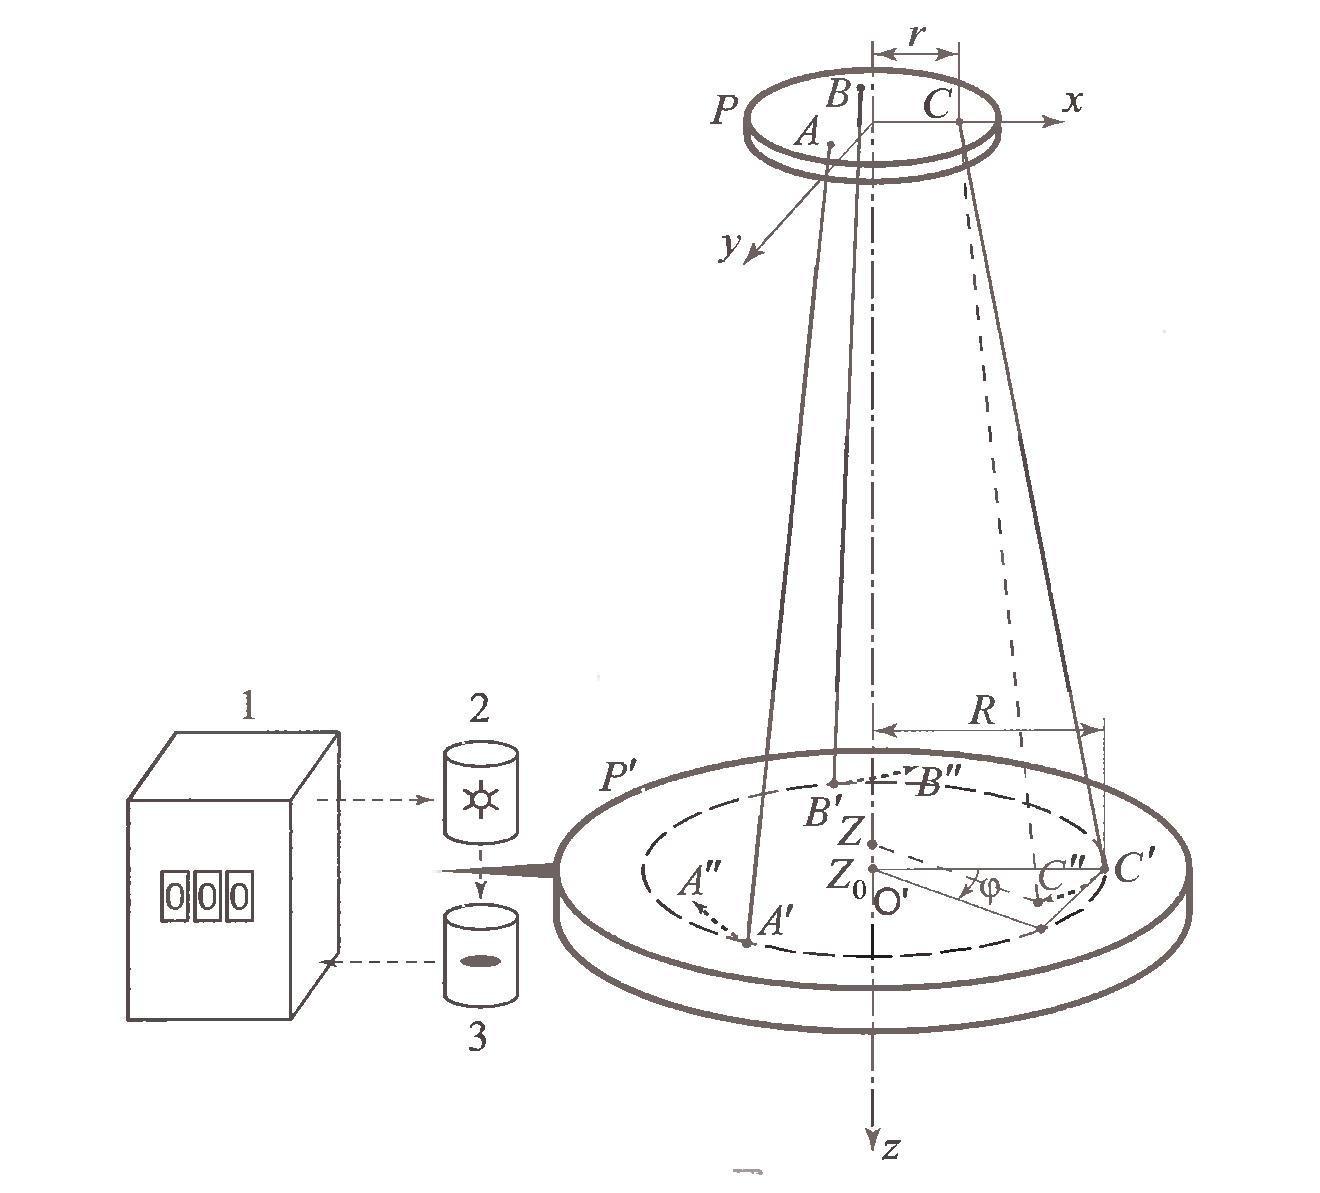
\includegraphics[width=0.95\linewidth]{1.2.3 ustan.png}
		\caption{Физический маятник}\label{risunok}
	\end{wrapfigure}

	Для наших целей удобно использовать устройство, показанное на Рис. \ref{risunok} и называемое трифилярным подвесом. Оно состоит из укрепленной на некоторой высоте неподвижной платформы $P$ и подвешенной к ней на трех симметрично расположенных нитях $AA'$, $BB'$ и $CC'$, вращающейся платформы $P'$.

	Чтобы не вызывать дополнительных раскачиваний, лучше поворачивать верхнюю платформу, укрепленную на неподвижной оси. После поворота верхняя платформа остается неподвижной в течение всего процесса колебаний. После того, как нижняя платформа $P'$ оказывается повернутой на угол $\varphi$ относительно верхней платформы $P$ возникает момент сил, стремящийся вернуть нижнюю платформу в положение равновесия, при котором относительный поворот платформ отсутствует. В результате платформа совершает крутильные колебания.

	\noindent где $k = \frac{gRr}{4\pi^2z_0}$ -- величина, постоянная для данной установки.

	\section{Оборудование}
	Трифилярный подвес, секундомер, счетчик числа колебаний, набор тел, момент инерции которых надлежит измерить (диск, стержень, полный цилиндр и другие).
\newpage
\section{Измерения и обработка данных}
\subsection{Измерения параметров установки}
Геометрические параметры установки представлены в таблице 1, момент инерции пустой платформы (согласно таблице \ref{пустая}) равен:
\begin{equation}
I_{\text{платформы}} = 7.85 \pm 0.17 \text{г}\cdot \text{м}^2
\end{equation}
\begin{table} \label{геом} \caption{Геометрические параметры установки}
\begin{tabular}{|c|c|c|c|c|}
\hline 
$z_0$, мм& $R$, мм & r, мм & k, $\text{м}^2/\text{c}^2$ & $\sigma_k$, $\text{м}^2/\text{c}^2$ \\ 
\hline 
$2166.93 \pm 0.018$ & $114.6 \pm 0.5$ & $30.5 \pm 0.3$ & $0.40 \cdot 10^{-3}$ & $0.02 \cdot 10^{-3}$ \\ 
\hline 
\end{tabular} 
\end{table}


\begin{table} \label{пустая} \caption{Измерения момента инерции пустой платформы} \begin{tabular}{|c|c|c|c|c|c|c|} \hline N & $m_\text{груза}/\text{c}^2$, г & t, с & T, с & k, $\cdot 10^{-3}\text{м}^2/\text{c}^2$ & $m_\text{плат}, г$& $I_\text{тела}, \text{г}\cdot \text{м}^2$ \\ \hline 10 & 0 & 44 & 4.425 & 0.404 & 983 & 7.852 \\ \hline 10 & 0 & 44 & 4.422 & 0.404 & 983 & 7.841 \\ \hline 10 & 0 & 44 & 4.417 & 0.404 & 983 & 7.822 \\ \hline 11 & 0 & 48 & 4.423 & 0.404 & 983 & 7.846 \\ \hline 10 & 0 & 44 & 4.415 & 0.404 & 983 & 7.815 \\ \hline 10 & 0 & 44 & 4.411 & 0.404 & 983 & 7.801 \\ \hline 10 & 0 & 44 & 4.406 & 0.404 & 983 & 7.785 \\ \hline 10 & 0 & 44 & 4.402 & 0.404 & 983 & 7.772 \\ \hline \end{tabular} \end{table}


\subsection{Измерения моментов инерции разных тел}
\begin{table} \label{Диск} \caption{Измерение момента инерции диска} \begin{tabular}{|c|c|c|c|c|c|c|c|c|} \hline N & $m_\text{груза}$, г & t, с & T, с & k, $\cdot 10^{-3}\text{м}^2/\text{c}^2$ & $m_\text{плат}, г$ & $I_\text{системы}, \text{г}\cdot \text{м}^2$ &$I_\text{платформы}, \text{г}\cdot \text{м}^2$ & $I_\text{тела}, \text{г}\cdot \text{м}^2$ \\ \hline 10 & 590 & 39 & 3.958 & 0.404 & 993 & 10.013 & 7.817 & 2.197 \\ \hline 10 & 590 & 39 & 3.952 & 0.404 & 993 & 9.985 & 7.817 & 2.168 \\ \hline 10 & 590 & 39 & 3.95 & 0.404 & 993 & 9.975 & 7.817 & 2.159 \\ \hline 10 & 590 & 39 & 3.949 & 0.404 & 993 & 9.97 & 7.817 & 2.153 \\ \hline 10 & 590 & 39 & 3.948 & 0.404 & 993 & 9.963 & 7.817 & 2.146 \\ \hline 10 & 590 & 39 & 3.947 & 0.404 & 993 & 9.96 & 7.817 & 2.143 \\ \hline \end{tabular} \end{table}

\begin{table} \label{Цилиндр} \caption{Измерение момента инерции цилиндра} \begin{tabular}{|c|c|c|c|c|c|c|c|c|} \hline N & $m_\text{груза}$, г & t, с & T, с & k, $\cdot 10^{-3}\text{м}^2/\text{c}^2$ & $m_\text{плат}, г$ & $I_\text{системы}, \text{г}\cdot \text{м}^2$ &$I_\text{платформы}, \text{г}\cdot \text{м}^2$ & $I_\text{тела}, \text{г}\cdot \text{м}^2$ \\ \hline 10 & 772 & 42 & 4.208 & 0.404 & 993 & 12.622 & 7.817 & 4.805 \\ \hline 11 & 772 & 46 & 4.205 & 0.404 & 993 & 12.6 & 7.817 & 4.783 \\ \hline 11 & 772 & 46 & 4.202 & 0.404 & 993 & 12.584 & 7.817 & 4.767 \\ \hline 10 & 772 & 41 & 4.2 & 0.404 & 993 & 12.568 & 7.817 & 4.752 \\ \hline 10 & 772 & 41 & 4.2 & 0.404 & 993 & 12.57 & 7.817 & 4.753 \\ \hline 10 & 772 & 41 & 4.195 & 0.404 & 993 & 12.542 & 7.817 & 4.725 \\ \hline \end{tabular} \end{table}

\begin{table} \label{Параллелепипед} \caption{Измерение момента инерции параллелепипеда} \begin{tabular}{|c|c|c|c|c|c|c|c|c|} \hline N & $m_\text{груза}$, г & t, с & T, с & k, $\cdot 10^{-3}\text{м}^2/\text{c}^2$ & $m_\text{плат}, г$ & $I_\text{системы}, \text{г}\cdot \text{м}^2$ &$I_\text{платформы}, \text{г}\cdot \text{м}^2$ & $I_\text{тела}, \text{г}\cdot \text{м}^2$ \\ \hline 13 & 1077 & 49 & 3.782 & 0.404 & 993 & 11.957 & 7.817 & 4.14 \\ \hline 13 & 1077 & 49 & 3.776 & 0.404 & 993 & 11.92 & 7.817 & 4.103 \\ \hline 10 & 1077 & 37 & 3.78 & 0.404 & 993 & 11.945 & 7.817 & 4.128 \\ \hline 10 & 1077 & 37 & 3.777 & 0.404 & 993 & 11.925 & 7.817 & 4.108 \\ \hline 19 & 1077 & 72 & 3.794 & 0.404 & 993 & 12.031 & 7.817 & 4.214 \\ \hline 10 & 1077 & 37 & 3.791 & 0.404 & 993 & 12.012 & 7.817 & 4.195 \\ \hline \end{tabular} \end{table}


Измерения момента инерции диска представлены в таблице \ref{Диск}, согласно теоретическому расчету из геометрических размеров диска: $I_\text{диск}=2.11 \text{г}\cdot \text{м}^2$. Из полученных данных: $I_\text{диск}=2.17 \pm 0.07 \text{г}\cdot \text{м}^2$. Это подтверждает правильность метода измерения.

Измерения момента инерции цилиндра представлены в таблице \ref{Цилиндр}, согласно теоретическому расчету из геометрических размеров цилиндра: $I_\text{цилиндр}=4.64 \text{г}\cdot \text{м}^2$. Из полученных данных: $I_\text{цилиндр}=4.79 \pm 0.09 \text{г}\cdot \text{м}^2$. Это подтверждает правильность метода измерения.

Измерения момента инерции параллелепипеда представлены в таблице \ref{Параллелепипед}, согласно теоретическому расчету из геометрических размеров параллелепипеда: $I_\text{кубоид}=4.02 \text{г}\cdot \text{м}^2$. Из полученных данных: $I_\text{кубоид}=4.14 \pm 0.04 \text{г}\cdot \text{м}^2$. Это подтверждает правильность метода измерения.

\subsection{Проверка закона аддитивности момента инерции}
\begin{table} \label{Диск+цилиндр} \caption{Измерение момента инерции диска и цилиндра} \begin{tabular}{|c|c|c|c|c|c|c|c|c|} \hline N & $m_\text{груза}$, г & t, с & T, с & k, $\cdot 10^{-3}\text{м}^2/\text{c}^2$ & $m_\text{плат}, г$ & $I_\text{системы}, \text{г}\cdot \text{м}^2$ &$I_\text{платформы}, \text{г}\cdot \text{м}^2$ & $I_\text{тела}, \text{г}\cdot \text{м}^2$ \\  \hline 21 & 1362 & 83 & 3.953 & 0.404 & 993 & 14.86 & 7.817 & 7.043 \\ \hline 11 & 1362 & 43 & 3.91 & 0.404 & 993 & 14.813 & 7.817 & 6.996 \\ \hline 11 & 1362 & 43 & 3.943 & 0.404 & 993 & 14.786 & 7.817 & 6.969 \\ \hline 11 & 1362 & 43 & 3.91 & 0.404 & 993 & 14.76 & 7.817 & 6.944 \\ \hline 16 & 1362 & 62 & 3.936 & 0.404 & 993 & 14.734 & 7.817 & 6.917 \\ \hline 12 & 1362 & 47 & 3.91 & 0.404 & 993 & 14.678 & 7.817 & 6.861 \\ \hline 10 & 1362 & 39 & 3.928 & 0.404 & 993 & 14.672 & 7.817 & 6.855 \\ \hline \end{tabular} \end{table}

Согласно таблице \ref{Диск+цилиндр}: $I_\text{диск+цилиндр}=6.92 \pm 0.03 \text{г}\cdot \text{м}^2$. Согласно измерениям моментов инерции тел по отдельности:
$I_\text{диск+цилиндр}=6.97 \pm 0.11 \text{г}\cdot \text{м}^2$.
Из чего следует справедливость закона аддитивности момента инерции.


\subsection{Измерение зависимости момента инерции диска от раздвижения его половинок}
\begin{table} \label{Половинки} \caption{Измерение момента инерции диска при движении половинок} \begin{tabular}{|c|c|c|c|c|c|c|c|c|c|} \hline N & $m_\text{груза}$, г & t, с & T, с & k, $\cdot 10^{-3}\text{м}^2$ & $m_\text{плат}, г$ & $I_\text{системы}, \text{г}\cdot \text{м}^2$ &$I_\text{платформы}, \text{г}\cdot \text{м}^2$ & $I_\text{тела}, \text{г}\cdot \text{м}^2$ & h, см \\ \hline 30 & 1528 & 91 & 3.061 & 0.404 & 993 & 9.536 & 7.817 & 1.72 & 0 \\ \hline 32 & 1528 & 98 & 3.067 & 0.404 & 993 & 9.575 & 7.817 & 1.758 & 0 \\ \hline 31 & 1528 & 95 & 3.074 & 0.404 & 993 & 9.616 & 7.817 & 1.8 & 1 \\ \hline 30 & 1528 & 93 & 3.12 & 0.404 & 993 & 9.907 & 7.817 & 2.09 & 1 \\ \hline 30 & 1528 & 94 & 3.157 & 0.404 & 993 & 10.147 & 7.817 & 2.33 & 2 \\ \hline 34 & 1528 & 109 & 3.21 & 0.404 & 993 & 10.486 & 7.817 & 2.669 & 2 \\ \hline 35 & 1528 & 114 & 3.275 & 0.404 & 993 & 10.916 & 7.817 & 3.099 & 3 \\ \hline 30 & 1528 & 100 & 3.338 & 0.404 & 993 & 11.338 & 7.817 & 3.521 & 3 \\ \hline 31 & 1528 & 106 & 3.429 & 0.404 & 993 & 11.97 & 7.817 & 4.154 & 4 \\ \hline \end{tabular} \end{table}
По данным из таблицы \ref{Половинки} построим график зависимости момента инерции диска от расстояния от каждой из половинок до центра платформы. График на рисунке \ref{график} 


\begin{figure}[h!]
\begin{center}
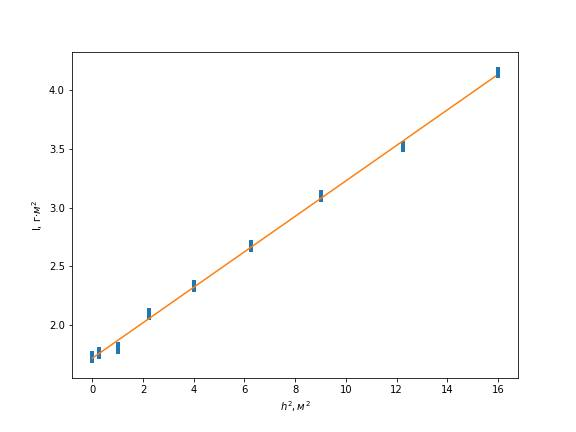
\includegraphics[width=\textwidth]{graph123.jpg}
\end{center}
\caption{График зависимости момента инерции диска от квадрата расстояния от каждой из половинок до центра платформы} \label{график}
\end{figure}


По наклону графика можно определить массу диска (в соотвествии в теоремой Гюйгенса-Штейнера): $m = 1.52 \pm 0.02 $кг, по отклонению найти момент инерции диска: $I = 1.69 \pm 0.02 \text{г}\cdot \text{м}^2$. Что согласуется с измеренной массой ($m = 1.53 \pm 0.02 $кг), теоретическим расчетом момента инерции: $I = 1.53 \pm 0.02 \text{г}\cdot \text{м}^2$

\section{Обсуждение результатов}
Величина момента инерции, определенная с помощью трифилярного подвеса с довольно большой точностью совпадает с теоретическими предсказаниями. Большая точность обеспечивается малой погрешностью измерения времени, а также выбором условий, при которых крутильные колебания подвеса можно считать слабозатухающими.
Основной вклад в погрешность измерения момента инерции внесла погрешность косвенного измерения. Данную погрешность можно уменьшить, если более точно определить параметры установки.
Была получена зависимость $ I(h^{2}) $, аппроксимируемая прямой, что подтверждает теоретические данные.
\section{Вывод}
		
		Мы экспериментально доказали аддитивность моментов инерции с помощью различных тел.

        
		
		Полученная зависимость $I(h^2)$ аппроксимируется линейной зависимостью, что подвтерждает формулу Гюйгенса-Штейнера ($I = I_c + Mh^2$, где $I$ -- момент инерции тела, $I_c$ --момент инерции тела относительно центра, $M$ -- масса тела, а $h$ -- расстояние между двумя осями, в нашем случае -- между осью вращения и половинками диска).
		
\end{document}

\end{document}
